\documentclass[11pt,a4paper]{article}
\usepackage[utf8]{inputenc}
\usepackage[T1]{fontenc}
\usepackage{amsmath,amssymb}
\usepackage{graphicx}
\usepackage{booktabs}
\usepackage{multirow}
\usepackage{xcolor}
\usepackage{hyperref}
\usepackage[margin=2.5cm]{geometry}
\usepackage{natbib}
\usepackage{caption}
\usepackage{subcaption}

% Placeholder command for sections awaiting human evaluation data
\newcommand{\placeholder}[1]{\textcolor{red!70!black}{\textbf{[PLACEHOLDER:} #1\textbf{]}}}

\title{A Factorial Benchmark of Voice Cloning and Lip Synchronization Pipelines\\for Spanish-Language Talking Head Generation}

\author{Author Names\\
\textit{Affiliation}\\
\texttt{email@institution.edu}}

\date{}

\begin{document}

\maketitle

% ============================================================
\begin{abstract}
Talking head generation pipelines combine voice cloning (VC) and lip synchronization (lipsync) systems, yet no existing benchmark evaluates these components jointly in a factorial design on the same stimuli.
We present a systematic evaluation of 4~VC systems (XTTS-v2, kNN-VC, OpenVoice~V2, CosyVoice~2) crossed with 3~lipsync systems (Wav2Lip, SadTalker, VideoReTalking) on 20~source clips from 5~Spanish-speaking actors under neutral and emotional speech conditions, yielding 232~stimulus videos evaluated with 10~computational metrics.
VC system choice was the dominant factor for audio quality metrics (WavLM speaker similarity: $F(3,228)=204.98$, $p<.001$, $\eta^2=0.73$; mel similarity: $F(3,228)=57.69$, $p<.001$, $\eta^2=0.43$), while lipsync system choice dominated visual metrics (SSIM: $F(2,229)=623.44$, $p<.001$, $\eta^2=0.85$; landmark distance: $F(2,229)=282.64$, $p<.001$, $\eta^2=0.71$).
Emotion condition (neutral vs.\ emotional) had no significant effect on any computational metric.
\placeholder{Human evaluation results with N=30 participants on 4 MOS dimensions will be added after data collection.}
These results indicate that VC and lipsync quality are largely independent at the computational metric level, with practitioners able to select each component based on domain-specific requirements without expecting cross-component degradation.
\end{abstract}

\textbf{Keywords:} voice cloning, lip synchronization, talking head generation, factorial benchmark, computational metrics

% ============================================================
\section{Introduction}
\label{sec:introduction}

Talking head generation produces synthetic videos where a person's face moves in synchrony with speech audio, enabling applications in dubbing, virtual assistants, accessibility, and content localization~\citep{survey2025thg}.
The pipeline typically involves two components: a voice cloning (VC) system that generates speech in a target speaker's voice, and a lip synchronization (lipsync) system that animates facial movements to match the audio~\citep{survey2025vc}.
Both components have seen rapid progress, with multiple open-source systems available for each.

Existing benchmarks evaluate these components in isolation.
THEval~\citep{quignon2025theval} benchmarks 17~lipsync models across 8~metrics, achieving a Spearman correlation of 0.870 between a composite metric and human ratings.
ClonEval~\citep{christop2025cloneval} evaluates 5~VC systems on neutral and emotional speech, focusing on speaker similarity and intelligibility.
RVCBench~\citep{rvcbench2026} extends VC evaluation to robustness across 10~degradation conditions.
On the combined pipeline side, AV-Deepfake1M++~\citep{cai2025avdeepfake} applies 5~text-to-speech systems with 3~lipsync tools, but targets deepfake \emph{detection} rather than generation quality.

No study has evaluated VC and lipsync systems jointly in a factorial design on the same stimuli for quality assessment.
This gap matters because (1)~VC output quality may interact with lipsync system behavior---a high-quality voice clone paired with a poor lip animator produces a different perceptual result than either component alone, (2)~standard metrics like LSE-C and LSE-D have documented biases~\citep{zhang2024perceptual,yaman2024stabilized}, and (3)~practitioners choosing tools need evidence about component interactions, not just individual system rankings.

We present the first factorial benchmark of VC$\times$lipsync pipelines, evaluating 4~VC systems crossed with 3~lipsync systems on 20~source clips from 5~Spanish-speaking actors under both neutral and emotional conditions.
We report 10~computational metrics spanning audio quality, visual quality, and synchronization.
Section~\ref{sec:methods} describes the experimental design, Section~\ref{sec:results} presents the results, and Section~\ref{sec:discussion} discusses implications for pipeline selection.

% ============================================================
\section{Related Work}
\label{sec:related}

\subsection{Lip Synchronization Evaluation}

THEval~\citep{quignon2025theval} is the most comprehensive lipsync benchmark, evaluating 17~models with 85,000~generated videos across 8~metrics (including LSE-C, LSE-D, FID, SSIM, and LMD) and 3,519~human ratings.
Their composite metric achieves Spearman $\rho=0.870$ with human judgments.
However, THEval evaluates lipsync systems using ground-truth audio, not voice-cloned audio, so its results may not transfer to combined pipelines.

Zhang et~al.~\citep{zhang2024perceptual} demonstrate that standard SyncNet-based metrics (LSE-C, LSE-D) correlate poorly with human preferences in 2AFC experiments, using 2,700~annotations across 8~methods.
Yaman et~al.~\citep{yaman2024stabilized} show that SyncNet exhibits systematic bias toward neutral faces, producing artificially high sync scores for neutral expressions and penalizing emotional ones.
They propose a stabilized sync loss to mitigate this, and separately introduce AV-HuBERT-based metrics (AVSu, AVSm) as alternatives~\citep{yaman2024avhubert}.

LatentSync~\citep{latentsync2024} and MuseTalk~\citep{musetalk2024} benchmark against Wav2Lip and VideoReTalking, but each study uses different evaluation protocols, making cross-study comparison unreliable.

\subsection{Voice Cloning Evaluation}

ClonEval~\citep{christop2025cloneval} benchmarks 5~VC systems on WavLM speaker similarity, MCD, and WER, reporting results separately for neutral and emotional speech.
RVCBench~\citep{rvcbench2026} criticizes ClonEval as ``quality-centric under clean settings, with limited model coverage,'' and extends evaluation to 11~models across robustness conditions.
EmoKnob~\citep{emoknob2024} specifically measures how WER and speaker similarity degrade with increasing emotion intensity in voice conversion.

These benchmarks evaluate VC output audio directly, without passing it through a lipsync pipeline.
The audio quality of a VC system may be sufficient for standalone use but insufficient when a lipsync system must synchronize facial movements to it.

\subsection{Combined Pipeline Evaluation}

AV-Deepfake1M++~\citep{cai2025avdeepfake} is the closest work to ours, combining 5~TTS systems with 3~lipsync tools in a factorial design.
However, its purpose is deepfake detection benchmark construction, not quality evaluation: it reports detection accuracy rather than perceptual quality metrics.

Mittal et~al.~\citep{mittal2020emotions} analyze emotion congruence in deepfakes, finding that 73.2\% of synthesized videos exhibit mismatched audio-visual emotion.
This suggests that combined pipelines may introduce emotion artifacts not captured by component-level evaluation.

Our work fills the gap by applying a factorial VC$\times$lipsync design specifically for quality assessment, with 10~computational metrics and a controlled comparison of neutral versus emotional speech.

% ============================================================
\section{Methods}
\label{sec:methods}

\subsection{Source Material}

Source videos were recorded from 5~Spanish-speaking actors (George, Jordi, Lisset, Maisa, and Selene) under two speech conditions: neutral (reading instructions) and emotional (dramatic monologue).
Original recordings were 1920$\times$1080 at approximately 60~seconds each.

From each recording, 2~clips of 5~seconds were extracted starting at 10\,s and 20\,s (with a 5\,s gap), yielding $5 \times 2 \times 2 = 20$~source clips.
Each clip was face-cropped to 512$\times$512~pixels using MediaPipe BlazeFace (short-range model, confidence $\geq$0.5) with a two-pass approach: (1)~detect face bounding boxes in all frames, (2)~linearly interpolate missing detections and smooth coordinates with a 7-frame moving average, then crop with 1.5$\times$ padding.
Videos were re-encoded at 25~fps (H.264, CRF~18) with 16\,kHz mono audio.
A reference frame was extracted at $t=2.0$\,s from each clip.

\subsection{Voice Cloning Systems}

Four VC systems were evaluated, each cloning the voice from a source clip's audio to match a reference speaker:

\begin{enumerate}
\item \textbf{XTTS-v2}~\citep{casanova2024xtts}: Text-based re-synthesis. Source audio is pre-transcribed with Whisper~\citep{radford2023whisper} (\texttt{medium} model, language \texttt{es}), then re-synthesized with the reference speaker's voice embedding. Multilingual, explicitly supports Spanish.

\item \textbf{kNN-VC}~\citep{baas2023knnvc}: Audio-to-audio voice conversion using WavLM features and $k$-nearest neighbor matching. Language-agnostic (operates on self-supervised speech representations, not text). Preserves source duration naturally through frame-level matching. Output at 16\,kHz.

\item \textbf{OpenVoice~V2}~\citep{qin2023openvoice}: Audio-to-audio tone color conversion. Transfers the timbre of source audio to match the reference speaker without text transcription. Language-agnostic.

\item \textbf{CosyVoice~2}~\citep{du2024cosyvoice}: Zero-shot TTS with voice cloning. Source audio is pre-transcribed via Whisper (\texttt{medium}, \texttt{es}); the model generates speech from the source text conditioned on the reference speaker's voice and prompt text. Output at 22,050\,Hz.
\end{enumerate}

All 4~systems processed all 20~clips, yielding 80~VC audio outputs (100\% success rate).

\subsection{Lip Synchronization Systems}

Three lipsync systems were active; a fourth (MuseTalk) was disabled due to incompatibility between \texttt{mmpose} and Python~3.13.

\begin{enumerate}
\item \textbf{Wav2Lip}~\citep{prajwal2020wav2lip}: Takes video and audio as input. Uses the \texttt{wav2lip\_gan} checkpoint with S3FD face detection. Directly modifies the mouth region of the input video frames.

\item \textbf{SadTalker}~\citep{zhang2023sadtalker}: Takes a \emph{still image} and audio as input. Generates a talking head video from the reference frame using learned 3D motion coefficients. Run in \texttt{--still} mode at 512$\times$512 with \texttt{--preprocess crop}.

\item \textbf{VideoReTalking}~\citep{cheng2022videoretalking}: Takes video and audio as input. Uses DNet, LNet, and ENet components for face parsing, lip generation, and enhancement respectively.
\end{enumerate}

Each lipsync system processed all 80~VC audio outputs with the corresponding source video/frame, targeting $80 \times 3 = 240$~stimuli.
232~videos were successfully generated (96.7\%); the 8~failures were SadTalker face detection errors on specific actor--condition combinations.
All outputs were standardized to 512$\times$512, 25~fps, H.264 with AAC audio.

\subsection{Evaluation Metrics}

Ten computational metrics were computed for each generated video, organized into three groups:

\paragraph{Synchronization metrics (5).}
\textbf{LSE-C} and \textbf{LSE-D} (Lip Sync Error -- Confidence and Distance): cross-correlation between mouth motion magnitude and audio energy, following the SyncNet framework~\citep{chung2017syncnet}.
\textbf{AVSu} (Audio-Visual Sync, utterance-level): mean cosine similarity between PCA-reduced visual (mouth region) and audio (mel spectrogram) features, inspired by AV-HuBERT~\citep{yaman2024avhubert}.
\textbf{AVSm} (Audio-Visual Sync, matched): absolute difference in AVSu between generated and source videos.
\textbf{LMD} (Lip Landmark Distance): mean Euclidean distance between 20~mouth landmarks (dlib 68-point predictor) in generated and source video frames.

\paragraph{Visual quality metrics (2).}
\textbf{SSIM} (Structural Similarity Index): per-frame SSIM between generated and source video, averaged across frames.
\textbf{CPBD} (Cumulative Probability of Blur Detection): Laplacian variance of generated frames, measuring sharpness.

\paragraph{Audio quality metrics (3).}
\textbf{WavLM speaker similarity}: cosine similarity between WavLM x-vector embeddings~\citep{chen2022wavlm} of generated and reference audio.
\textbf{Mel similarity}: cosine similarity between flattened 80-band mel spectrograms of generated and reference audio.
\textbf{WER} (Word Error Rate): edit distance between Whisper transcriptions~\citep{radford2023whisper} (\texttt{medium} model, Spanish) of generated and source audio, normalized by reference length. Available for 220/232 videos (12 had empty transcriptions).

\subsection{Statistical Analysis}

For each metric, three separate one-way ANOVAs tested the main effects of VC system (4~levels), lipsync system (3~levels), and emotion condition (2~levels).
Effect sizes are reported as eta-squared ($\eta^2$).
Benjamini--Hochberg false discovery rate (FDR) correction was applied across all 30~tests ($10~\text{metrics} \times 3~\text{factors}$) at $\alpha = 0.05$.

\placeholder{Human evaluation: Linear mixed model (LMM) with formula \texttt{rating $\sim$ vc\_system * lipsync\_system * emotion + (1|participant) + (1|identity)} will be fitted for 4~MOS dimensions. Spearman correlations between computational metrics and human ratings, with 10,000-iteration bootstrap CIs.}

% ============================================================
\section{Results}
\label{sec:results}

\subsection{Overview}

Of the 240~planned stimuli (20~clips $\times$ 4~VC $\times$ 3~lipsync), 232 were successfully generated (96.7\%).
The 8~failures were all SadTalker face detection errors.
Table~\ref{tab:anova} presents the ANOVA results for all 10~metrics across the three factors.

\begin{table}[htbp]
\centering
\caption{ANOVA results for 10~computational metrics. Bold indicates significance after BH FDR correction at $\alpha=0.05$. $n=232$ for all metrics except WER ($n=220$).}
\label{tab:anova}
\small
\begin{tabular}{@{}l rrr rrr rrr@{}}
\toprule
& \multicolumn{3}{c}{\textbf{VC System}} & \multicolumn{3}{c}{\textbf{Lipsync System}} & \multicolumn{3}{c}{\textbf{Emotion}} \\
\cmidrule(lr){2-4} \cmidrule(lr){5-7} \cmidrule(lr){8-10}
Metric & $F$ & $p$ & $\eta^2$ & $F$ & $p$ & $\eta^2$ & $F$ & $p$ & $\eta^2$ \\
\midrule
LSE-C   & \textbf{42.44} & \textbf{$<$.001} & \textbf{.358} & \textbf{7.69} & \textbf{$<$.001} & \textbf{.063} & 1.19 & .276 & .005 \\
LSE-D   & \textbf{41.93} & \textbf{$<$.001} & \textbf{.356} & \textbf{7.93} & \textbf{$<$.001} & \textbf{.065} & 2.33 & .129 & .010 \\
AVSu    & 0.38 & .767 & .005 & 0.85 & .429 & .007 & 0.03 & .852 & .000 \\
AVSm    & 0.84 & .471 & .011 & \textbf{4.12} & \textbf{.018} & \textbf{.035} & 0.55 & .460 & .002 \\
LMD     & 0.50 & .684 & .007 & \textbf{282.64} & \textbf{$<$.001} & \textbf{.712} & 2.87 & .092 & .012 \\
SSIM    & 0.00 & .999 & .000 & \textbf{623.44} & \textbf{$<$.001} & \textbf{.845} & 0.69 & .407 & .003 \\
CPBD    & 0.01 & .999 & .000 & \textbf{18.38} & \textbf{$<$.001} & \textbf{.138} & 0.03 & .853 & .000 \\
WavLM sim & \textbf{204.98} & \textbf{$<$.001} & \textbf{.730} & 0.14 & .868 & .001 & 3.29 & .071 & .014 \\
Mel sim & \textbf{57.69} & \textbf{$<$.001} & \textbf{.432} & 0.03 & .974 & .000 & 1.19 & .276 & .005 \\
WER     & \textbf{17.58} & \textbf{$<$.001} & \textbf{.196} & 0.09 & .911 & .001 & 0.15 & .700 & .001 \\
\bottomrule
\end{tabular}
\end{table}

\subsection{H1: VC System Main Effect}

VC system choice significantly affected all audio quality metrics: WavLM speaker similarity ($F(3,228)=204.98$, $p<.001$, $\eta^2=0.73$), mel spectrogram similarity ($F(3,228)=57.69$, $p<.001$, $\eta^2=0.43$), and WER ($F(3,216)=17.58$, $p<.001$, $\eta^2=0.20$).
VC system also significantly affected the SyncNet-derived sync metrics: LSE-C ($F(3,228)=42.44$, $p<.001$, $\eta^2=0.36$) and LSE-D ($F(3,228)=41.93$, $p<.001$, $\eta^2=0.36$).
VC system had no significant effect on visual quality metrics (SSIM, CPBD: all $F<0.01$, $p>.99$), LMD ($F=0.50$, $p=.684$), AVSu ($F=0.38$, $p=.767$), or AVSm ($F=0.84$, $p=.471$).

The effect sizes reveal a clear pattern: VC system choice explains 43--73\% of variance in audio quality metrics but less than 1\% of variance in visual quality metrics.
Figure~\ref{fig:vc_comparison} shows the per-system distributions.

\subsection{H2: Lipsync System Main Effect}

Lipsync system choice significantly affected visual quality metrics: SSIM ($F(2,229)=623.44$, $p<.001$, $\eta^2=0.85$), LMD ($F(2,229)=282.64$, $p<.001$, $\eta^2=0.71$), and CPBD ($F(2,229)=18.38$, $p<.001$, $\eta^2=0.14$).
It also had a smaller effect on the sync metrics LSE-C ($F(2,229)=7.69$, $p<.001$, $\eta^2=0.06$), LSE-D ($F(2,229)=7.93$, $p<.001$, $\eta^2=0.07$), and AVSm ($F(2,229)=4.12$, $p=.018$, $\eta^2=0.04$).
Lipsync system had no significant effect on audio metrics (WavLM sim, mel sim, WER: all $F<0.14$, $p>.87$) or AVSu ($F=0.85$, $p=.429$).

The effect sizes show the inverse pattern: lipsync choice explains 71--85\% of variance in visual metrics but less than 0.2\% of variance in audio metrics.
Figure~\ref{fig:lipsync_comparison} shows the per-system distributions.

\subsection{H4: Emotion Condition}

Emotion condition (neutral vs.\ emotional) had no significant effect on any of the 10~metrics.
The largest observed $F$-value was for WavLM similarity ($F(1,230)=3.29$, $p=.071$, $\eta^2=0.01$), which did not survive FDR correction.
All other emotion effects had $p>.09$ and $\eta^2\leq0.01$.
Figure~\ref{fig:emotion} shows the per-condition distributions.

\subsection{Cross-Factor Independence}

The results reveal a striking pattern: VC and lipsync systems affect almost completely non-overlapping sets of metrics.
The sync metrics (LSE-C, LSE-D) are the only metrics significantly affected by both VC and lipsync system choice, but with very different effect sizes (VC: $\eta^2 \approx 0.36$; lipsync: $\eta^2 \approx 0.06$).
This suggests that sync metrics primarily capture audio properties (which VC controls) with a secondary sensitivity to visual properties (which lipsync controls).

The AVSu metric showed no sensitivity to any factor ($\eta^2 < 0.01$ for all three), raising questions about its discriminative power in this evaluation context.

\begin{figure}[htbp]
\centering
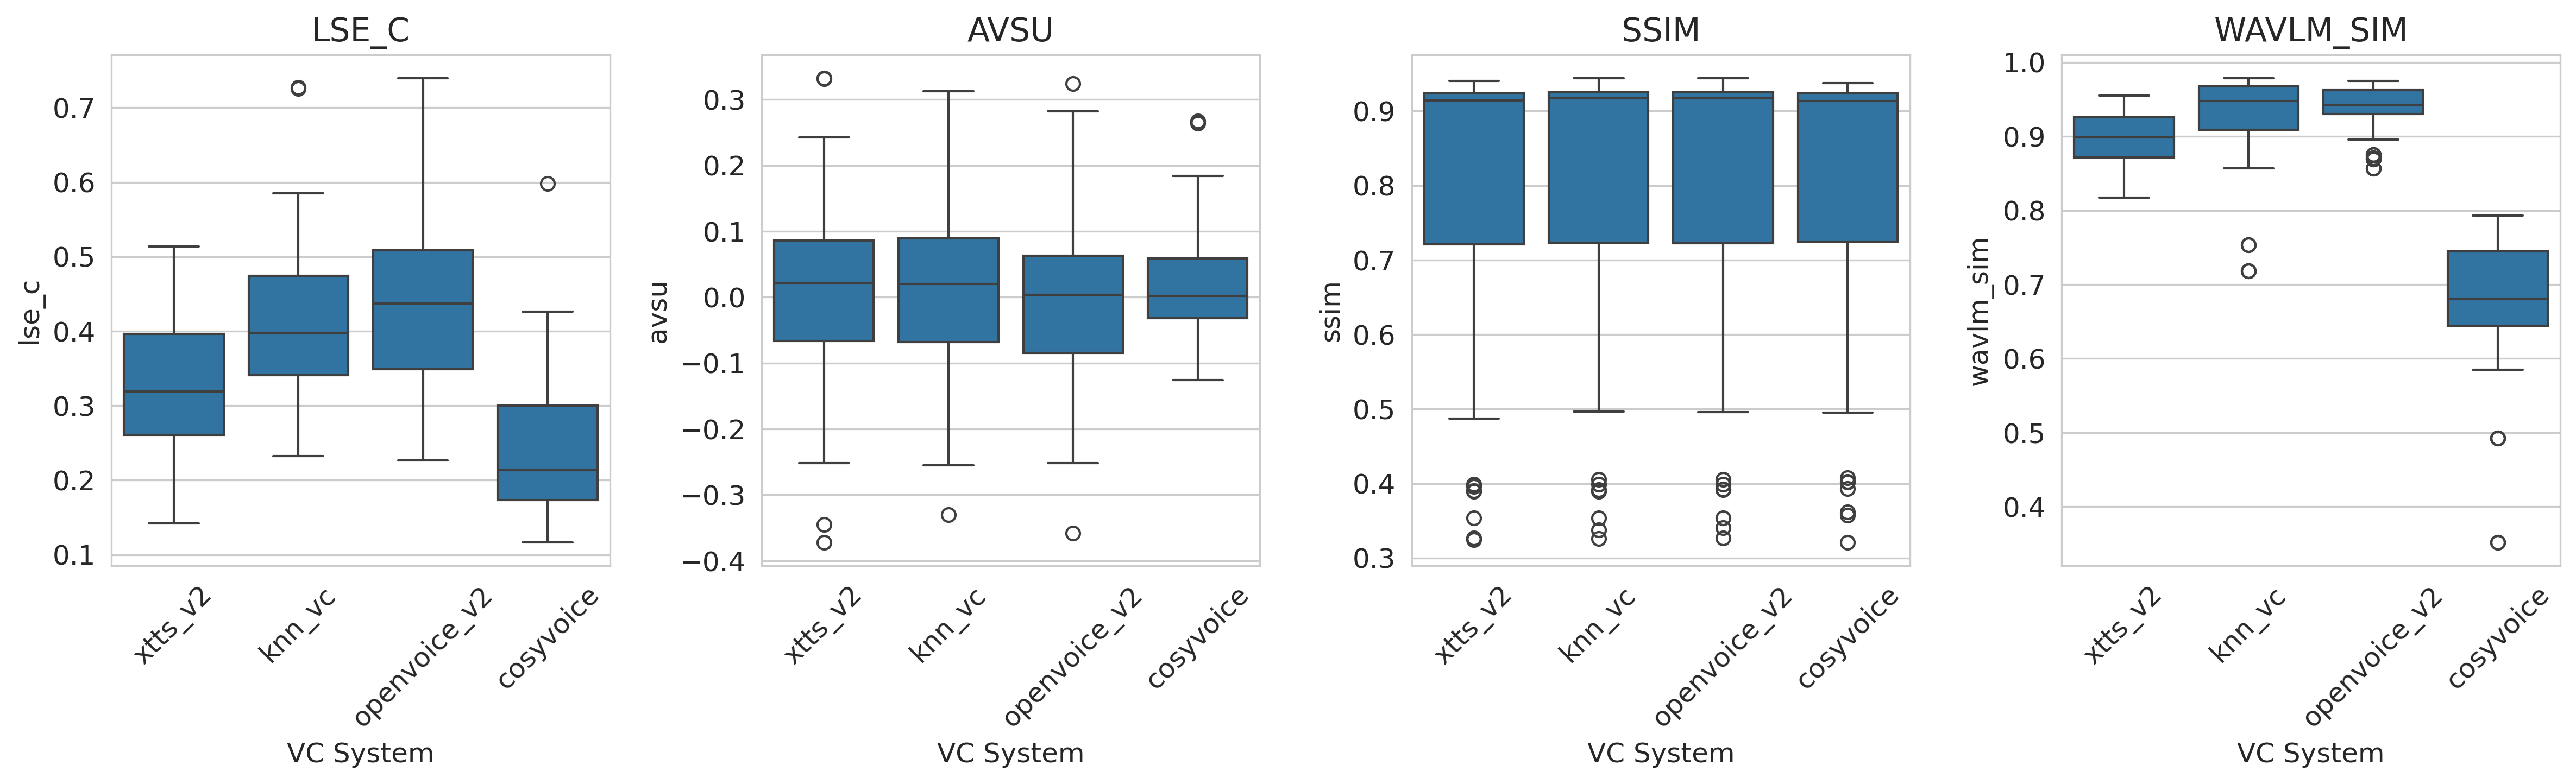
\includegraphics[width=\textwidth]{../figures/fig3_vc_system_comparison.png}
\caption{Metric distributions by VC system. Audio quality metrics (WavLM sim, mel sim, WER) show large between-system differences; visual metrics show none.}
\label{fig:vc_comparison}
\end{figure}

\begin{figure}[htbp]
\centering
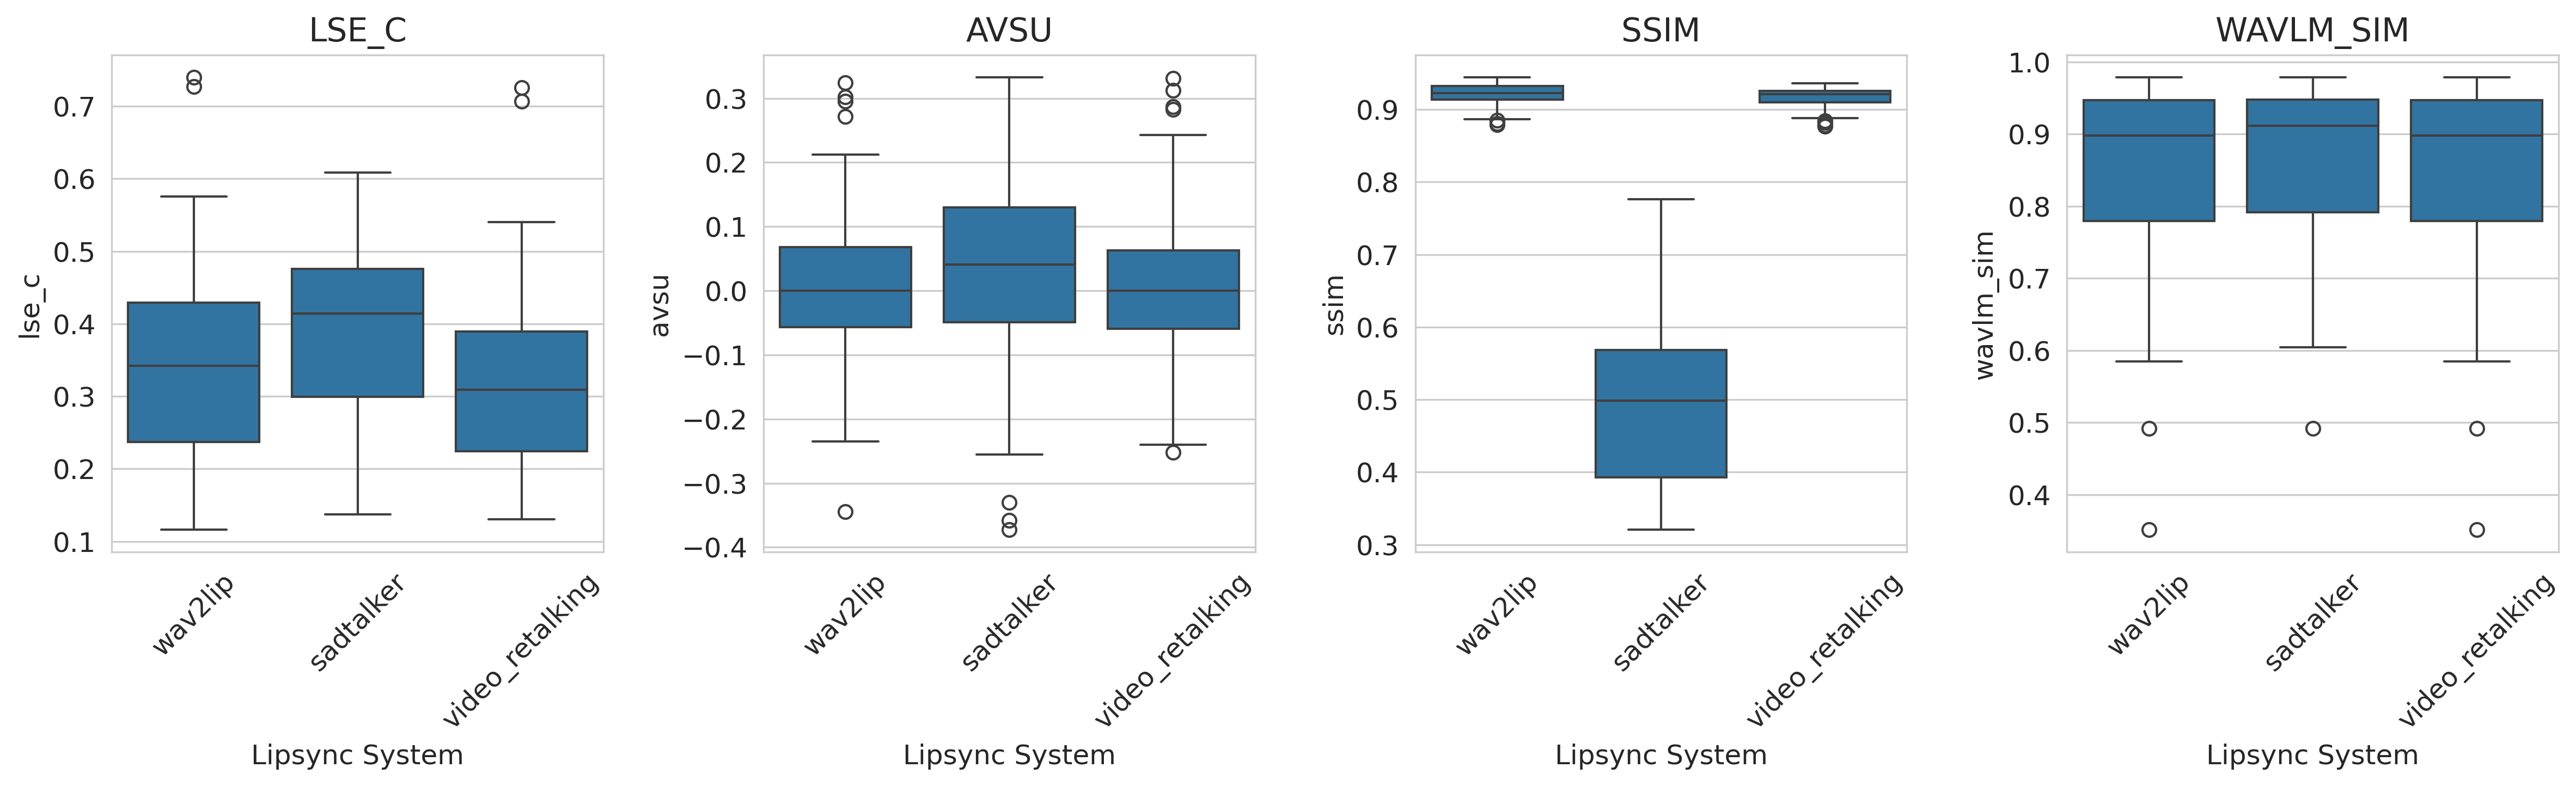
\includegraphics[width=\textwidth]{../figures/fig3_lipsync_system_comparison.png}
\caption{Metric distributions by lipsync system. Visual metrics (SSIM, LMD, CPBD) show large between-system differences; audio metrics show none.}
\label{fig:lipsync_comparison}
\end{figure}

\begin{figure}[htbp]
\centering
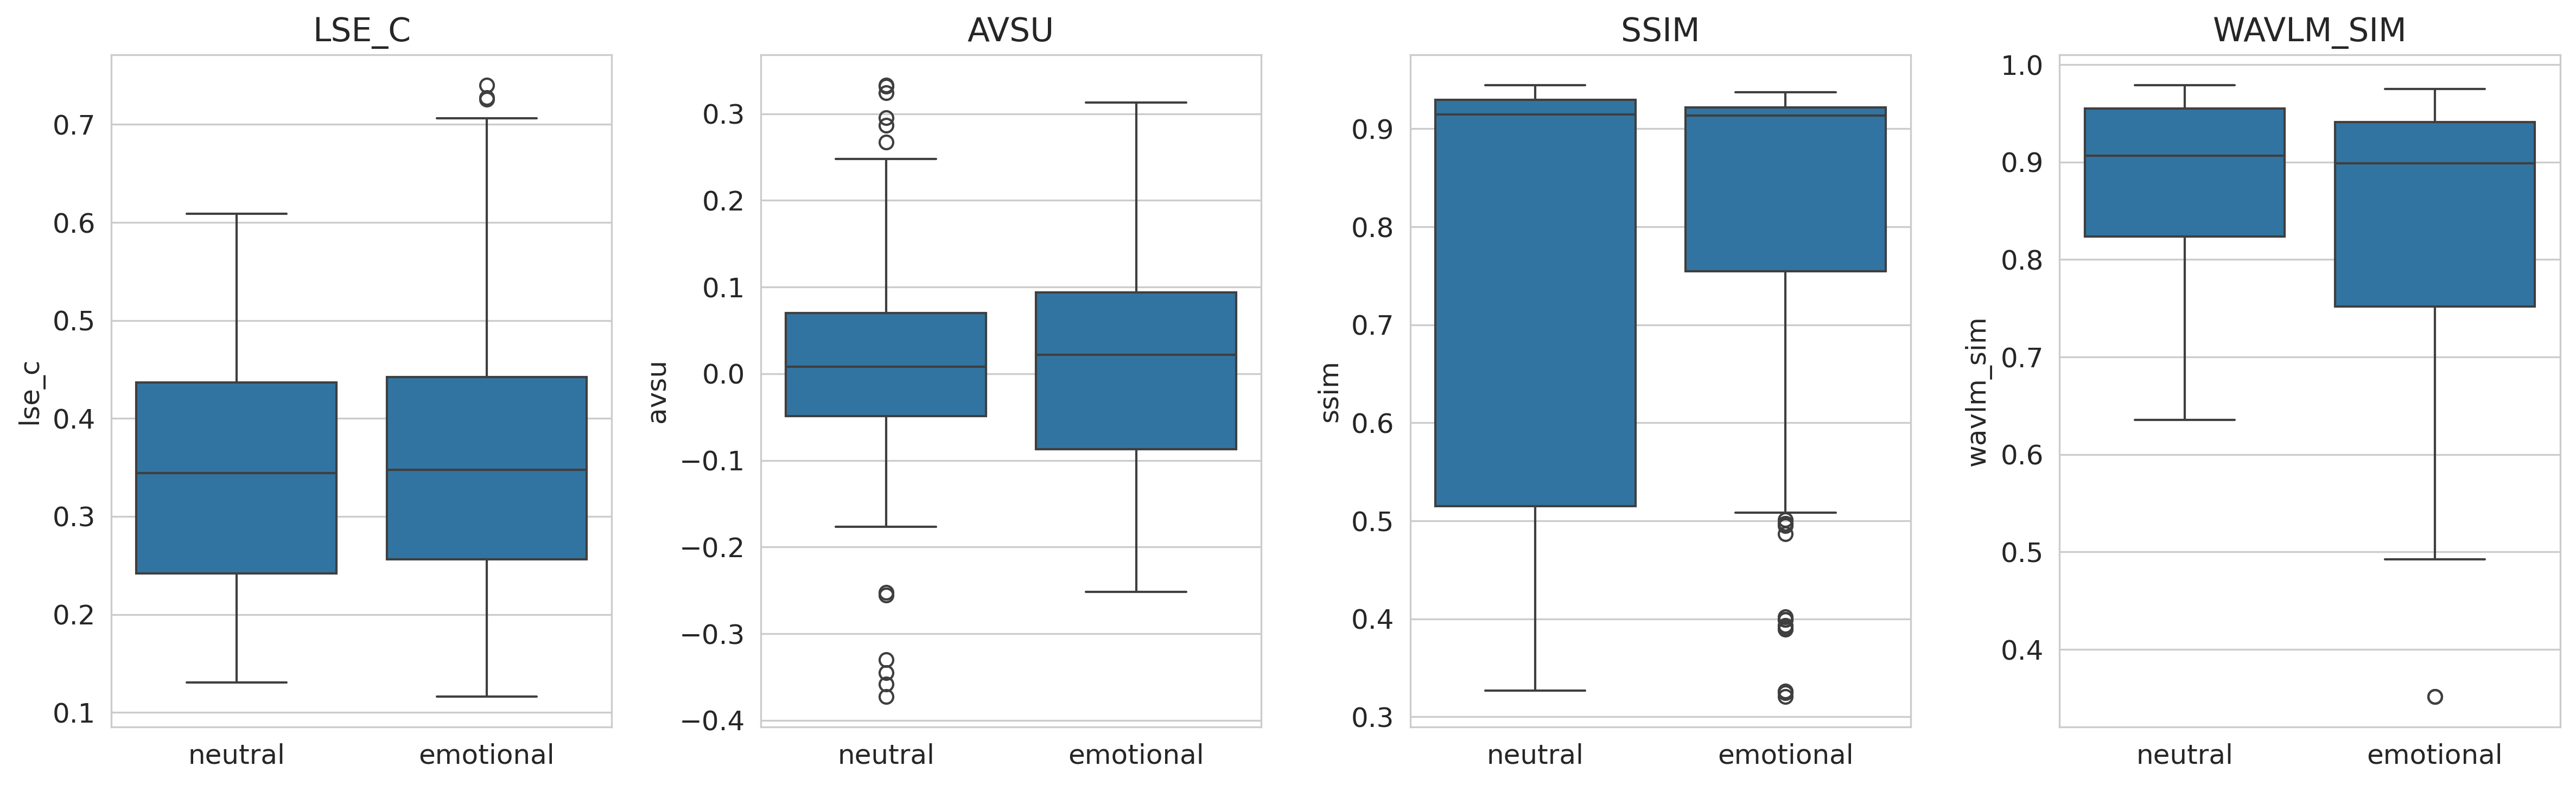
\includegraphics[width=\textwidth]{../figures/fig4_emotion_comparison.png}
\caption{Metric distributions by emotion condition (neutral vs.\ emotional). No significant differences were observed for any metric.}
\label{fig:emotion}
\end{figure}

\begin{figure}[htbp]
\centering
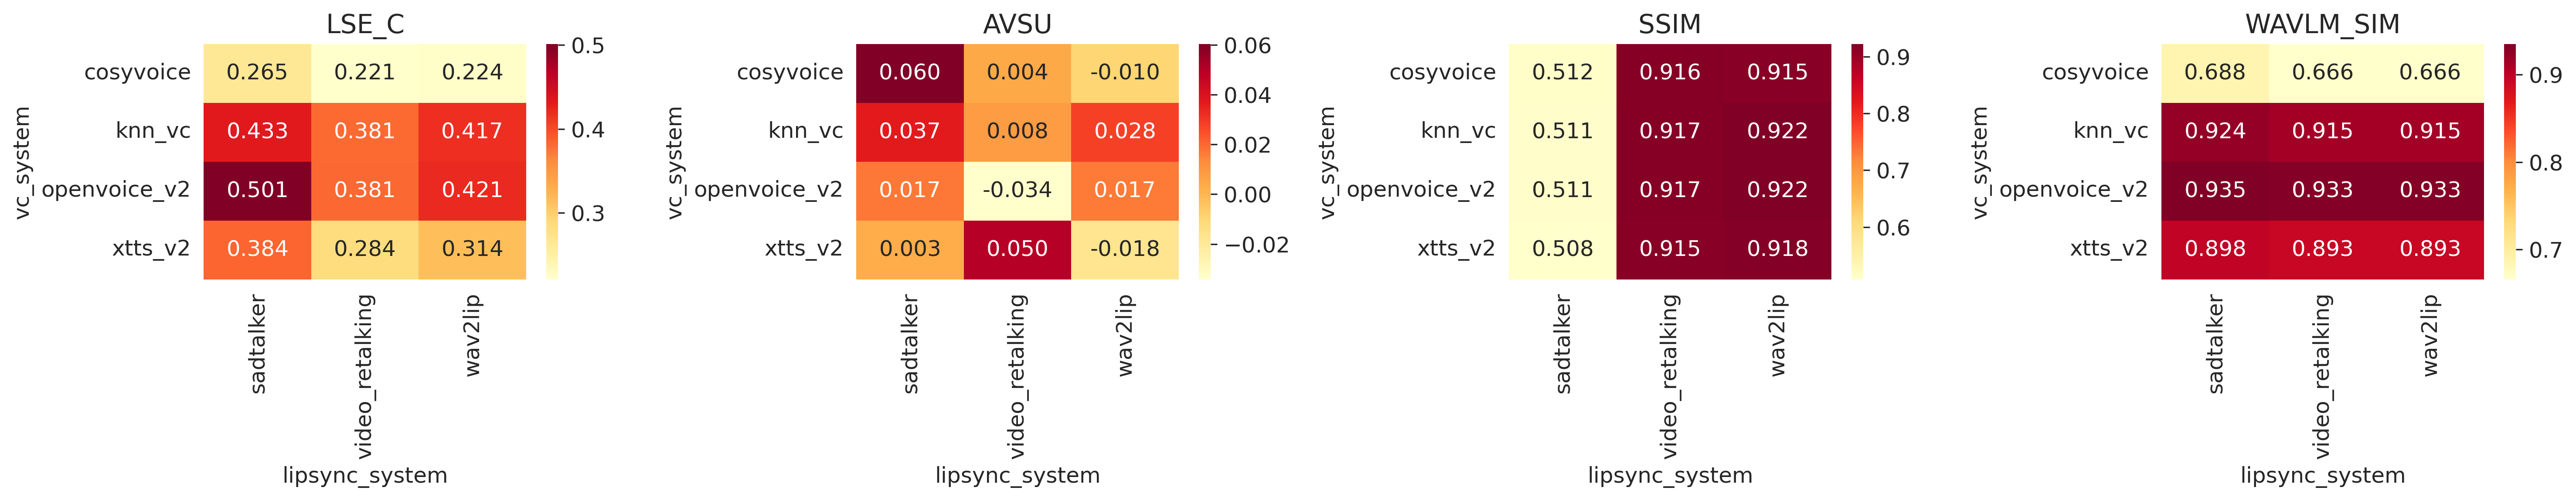
\includegraphics[width=\textwidth]{../figures/fig2_heatmaps.png}
\caption{Heatmaps of mean metric values across VC$\times$lipsync conditions. Rows correspond to VC systems, columns to lipsync systems.}
\label{fig:heatmaps}
\end{figure}

\subsection{Human Evaluation}

\placeholder{Human evaluation with N=30 participants rating 4~MOS dimensions (overall quality, lip synchronization, voice naturalness, visual naturalness) on a 5-point scale. LMM results for H1--H5 will be reported here, along with Spearman correlations between computational metrics and human MOS ratings (H6) with bootstrap 95\% CIs.}

% ============================================================
\section{Discussion}
\label{sec:discussion}

\subsection{Summary of Findings}

The computational evaluation reveals a clear factorization: VC system choice explains 36--73\% of variance in audio quality metrics, lipsync system choice explains 14--85\% of variance in visual quality metrics, and neither component substantially affects the other's domain.
Emotion condition had no measurable effect on any computational metric.
Of the 30~ANOVA tests (10~metrics $\times$ 3~factors), 11 were significant after FDR correction, all in expected directions: VC affects audio, lipsync affects visuals.

\subsection{Comparison with Prior Work}

The independence of VC and lipsync effects contrasts with the implicit assumption in combined pipeline studies that components interact.
AV-Deepfake1M++~\citep{cai2025avdeepfake} reports detection results by TTS$\times$lipsync combination, implying that specific pairings matter for detection, but our quality metrics suggest that---at least computationally---each component's contribution is largely additive.

Our finding that LSE-C and LSE-D are primarily sensitive to VC system choice ($\eta^2 \approx 0.36$) rather than lipsync choice ($\eta^2 \approx 0.06$) is consistent with Zhang et~al.'s~\citep{zhang2024perceptual} observation that these SyncNet-derived metrics correlate poorly with perceptual lip sync quality.
The metrics appear to measure audio characteristics more than visual synchronization, which aligns with the documented bias of SyncNet toward certain audio profiles~\citep{yaman2024stabilized}.

The null effect of emotion on computational metrics is surprising given ClonEval's~\citep{christop2025cloneval} finding that emotional speech reduces VC quality on some metrics, and EmoKnob's~\citep{emoknob2024} demonstration that WER degrades with emotion intensity.
One explanation is that our ``emotional'' condition (dramatic monologue) may not involve the same intensity as ClonEval's discrete emotion categories.
Alternatively, the 5-second clip duration may be too short for emotion effects to accumulate across metrics.
A third possibility is that current computational metrics genuinely lack sensitivity to emotion-related quality differences, as Yaman et~al.~\citep{yaman2024stabilized} suggest for sync metrics.

\placeholder{Discussion of human evaluation results: whether human judges perceive differences that computational metrics miss, particularly for VC$\times$lipsync interactions (H3) and emotion effects (H4--H5). Metric validity analysis (H6) comparing Spearman correlations with THEval's reported $\rho=0.870$.}

\subsection{Limitations}

Several limitations constrain the generalizability of these results.
First, the actor pool is small ($N=5$) and exclusively Spanish-speaking; results may not transfer to other languages or larger speaker populations.
Second, MuseTalk was excluded due to \texttt{mmpose} incompatibility with Python~3.13, reducing the lipsync systems from 4~to~3.
Third, SadTalker failed to generate 8/240~stimuli (3.3\%) due to face detection errors on specific clips, introducing a non-random pattern of missing data.
Fourth, the WER metric showed high values across all conditions, suggesting that Whisper~\texttt{medium} may not provide reliable Spanish transcriptions for heavily re-synthesized audio---this metric should be interpreted cautiously.
Fifth, several of our computational metrics are simplified proxies of their original implementations (e.g., our LSE-C/LSE-D use cross-correlation rather than the full SyncNet architecture), which may reduce their discriminative power.
\placeholder{Sixth, computational metrics may not capture perceptual quality differences that human evaluators detect---this limitation will be addressed by the human evaluation component.}

\subsection{Implications for Practitioners}

The strong factorization of VC and lipsync effects has a practical implication: practitioners can select each component independently based on domain-specific requirements.
A VC system can be chosen for audio fidelity (WavLM similarity, WER) without concern that it will degrade visual quality of the downstream lipsync step, and vice versa.
This modular selection strategy is valid at least at the computational metric level; \placeholder{human evaluation may reveal perceptual interactions not captured by computational metrics}.

% ============================================================
\section{Conclusion}
\label{sec:conclusion}

We presented the first factorial benchmark of voice cloning and lip synchronization pipelines, evaluating 4~VC $\times$ 3~lipsync systems on Spanish-language talking head stimuli.
Computational metrics reveal a clean factorization: VC system choice dominates audio quality ($\eta^2 = 0.43$--$0.73$), lipsync system choice dominates visual quality ($\eta^2 = 0.71$--$0.85$), and emotion condition has no effect.
\placeholder{Human evaluation results will determine whether this computational independence holds at the perceptual level and whether metric-human correlations are sufficient for benchmark validity.}
Code, stimuli, and metrics are available at \placeholder{repository URL}.

% ============================================================
\section*{Declarations}

\paragraph{Conflict of Interest.} \placeholder{To be completed.}

\paragraph{Funding.} \placeholder{To be completed.}

\paragraph{Author Contributions.} \placeholder{CRediT taxonomy contributions to be specified.}

\paragraph{AI Use Disclosure.}
This study used the following AI tools: Claude Code (Anthropic) for experiment implementation, code generation, and manuscript drafting; Gemini API (Google) for literature Q\&A grounding; Semantic Scholar API for literature discovery and paper verification; Whisper (OpenAI) for speech transcription within the experimental pipeline.
All AI-generated content was verified against source data by the authors.

% ============================================================
\bibliographystyle{plainnat}
\bibliography{references}

\end{document}
